% !TeX encoding = UTF-8
% !TeX program = XeLaTeX
% !TeX spellcheck = en_US

% Author : Shlw
% Description : TikZ Assignment
\documentclass{standalone}

\usepackage{tikz}

\begin{document}

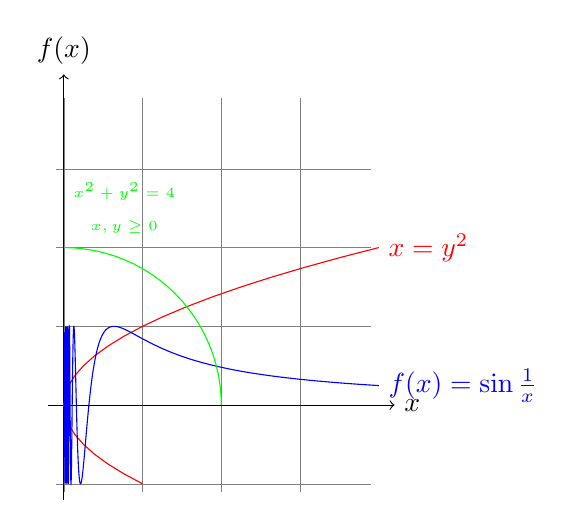
\begin{tikzpicture}[domain=0:4]
\draw[very thin,color=gray] (-0.1,-1.1) grid (3.9,3.9);

\draw[->] (-0.2,0) -- (4.2,0) node[right] {$x$};
\draw[->] (0,-1.2) -- (0,4.2) node[above] {$f(x)$};

\draw[color=red,domain=-1:2,variable=\y]  plot ({\y*\y},\y) 
    node[right] {$x=y^2$};
\draw[color=blue,domain=0.01:1,samples=2000] plot (\x,{sin(1/\x r)});
\draw[color=blue,domain=1:4] plot (\x,{sin(1/\x r)}) 
    node[right] {$f(x) = \sin\frac1x$};
\draw[color=green,domain=0:90] plot ({2*cos(\x)},{2*sin(\x)}) 
    node[right,align=center,yshift=0.5cm] {\tiny$x^2+y^2=4$\\\tiny$x,y\geq 0$};

\end{tikzpicture}

\end{document}
